\cxset{style13,
       chapter toc=true,
       toc image={}}
\chapter{The Special Environments Quotation and Quote}

\label{quotations}


\begin{figure}[p]
\centering
\fbox{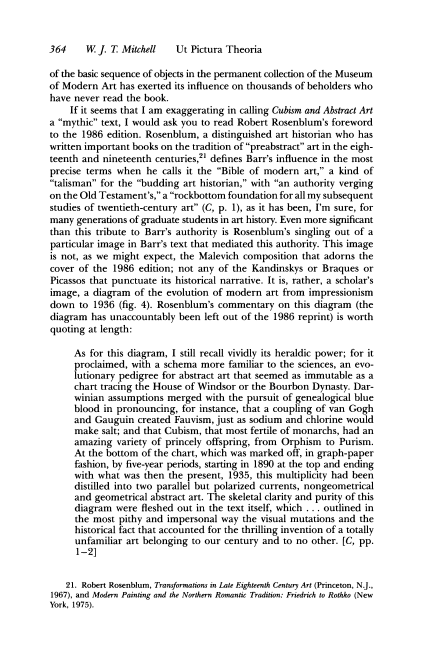
\includegraphics[width=0.9\linewidth]{./images/quotations-01.png}}
\caption{Many books have quotes flushed right.}
\label{frightquotation}
\end{figure}

\begin{figure}[p]
\centering
\fbox{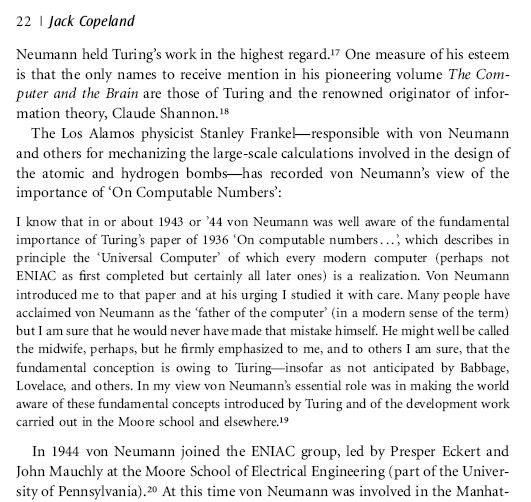
\includegraphics[width=0.9\linewidth]{./images/full-width-quotation.jpg}}
\caption[Sample quotation.]{Other books have the quotations full width, but in smaller font as shown above. the extract is from \textit{The Essential Turing}, Edited by B. Jack Copeland and  published by the Oxford University Press, 2004. }
\label{fullwidthquotation}
\end{figure}


\section{Quotation}
In the standard \LaTeXe\ classes the quotation and quote environment are defined by making use of the list environment. The main difference between the quotation and the quote environment is that the first line of the former is indented. The key value interface for the quotation environment is shown below and a similar one exists for the quotation environment:


\let\quotation\oquotation
\begin{quotation}
\lipsum[1]
\end{quotation}

The standard classes offer a very similar enevironment with the only difference the first line is not indented and is illustrated below:

\begin{quote}
\lipsum[1]
\end{quote}


\section{Key-value interface}\index{quotation!keys}

\keyval{quote above}{\marg{dim}}{Skip dimension for above quotation skip.}
\keyval{quote below}{\marg{dim}}{Skip dimension for below quotation skip.}
\keyval{quote parindent}{\marg{dim}}{Paragraph indentation.}
\keyval{quote parsep}{\marg{dim}}{Paragraph below skip.}
\keyval{quote left margin}{\marg{dim}}{Paragraph below skip.}
\keyval{quote right margin}{\marg{dim}}{Paragraph below skip.}
\vfill

\index{quotation!example}
\begin{tcblisting}{title=Quotation environment example,width=\textwidth}
\setquotation{%
  quotation above=36pt,
  quotation left margin=30pt,
  quotation right margin=0pt,
  quotation parsep=10pt,
  quotation font-size=\small\color{teal},
  quotation parindent=1em,
}
\lorem

\begin{quotation}
\lipsum[2-3]
\end{quotation}
\end{tcblisting}

\section{Quote}
This is the quote environment:
\begin{quote}
\lipsum[1-2]
\end{quote}


\section{Some commonly used styles}

Besides the centered quotation \fref{fullwidthquotation} shows a style
common in Oxford University Publications. This one is from \textit{The Essential Turing}, Edited by B. Jack Copeland and  published by the Oxford University Press, 2004. Perhaps indicative of the efforts of academic publications to keep costs down quotations are set at full width, but in smaller font. They both look good and keep the cost down by reducing the amount of paper required to print the book.

\topline

Von Neumann gave his engineers `On Computable Numbers' to read when, in
1946, he established his own project to build a stored-programme computer at
the Institute for Advanced Study.\textsuperscript{22} Julian Bigelow, von Neumann's chief engineer,
recollected:
\vspace*{-20pt}

\cxset{quotation example/.style={
  quotation above=0pt,
  quotation left margin=0pt,
  quotation right margin=0pt,
  quotation parsep=10pt,
  quotation font-size=\small\color{teal},
  quotation parindent=1em,
}}

\cxset{quotation turing/.style={
  quotation above=0pt,
  quotation left margin=0pt,
  quotation right margin=0pt,
  quotation parsep=10pt,
  quotation font-size=\small,
  quotation parindent=1em,
}}

\cxset{quotation theme/.code = \setquotation{quotation #1},
       quotation style/.code = \setquotation{quotation #1}}



\cxset{quotation theme = example}




\begin{quotation}

The person who really\ldots pushed the whole Weld ahead was von Neumann, because he
understood logically what [the stored-programme concept] meant in a deeper way than
anybody else\ldots The reason he understood it is because, among other things, he understood
a good deal of the mathematical logic which was implied by the idea, due to the
work of A. M. Turing\ldots in 1936-1937\ldots Turing's [universal] machine does not sound
much like a modern computer today, but nevertheless it was. It was the germinal
idea\ldots So\ldots [von Neumann] saw\ldots that \textsc{[ENIAC]} was just the first step, and that great
improvement would come.\textsuperscript{23}
\end{quotation}

\bottomline

Personally I like this style, especially for books that have a lot
of lengthy citations such as typically found in the humanities and
scientific fields.

\section{Theming}

To make things easier for the designer and to enable easy re-use of
styles we defined a theme key. You first define your keys via
the \cs{cxset} command and then you call it normally using the 
theme. You can extend it, if you like to use subthemes, such as 
quotation theme |quotation theme = example teal|. 

\begin{teX}
\cxset{quotation example/.style={
  quotation above=0pt,
  quotation left margin=0pt,
  quotation right margin=0pt,
  quotation parsep=10pt,
  quotation font-size=\small\color{teal},
  quotation parindent=1em,
}}
\cxset{quotation theme = example}
\end{teX}







